%===================================================================================
% Chapter: Analysis of Results
%===================================================================================
\chapter{Análisis de Resultados}\label{chapter:analysis-of-results}
%===================================================================================
El esquema de anotación y el modelo ontológico presentado en este trabajo, y por tanto el grafo de conocimiento generado a partir de ellos, tienen como objetivo fundamental asistir en el desarrollo de sistemas de descubrimiento de conocimiento en documentos escritos en lenguaje natural.

En este capítulo, se presenta el marco experimental diseñado para comprobar la efectividad del esquema de anotación y el modelo ontológico descrito en el capítulo \ref{chapter:annotation_model} y de la propuesta de solución presentada en el capítulo \ref{chapter:proposed-solution}.

\section{Marco experimental}
En esta investigación solo se trabajará con los artículos del corpus de \textit{Medline} en español, estos son procesados para eliminar las marcas específicas de \textit{HTML}\footnote{Siglas en inglés de \textit{\textbf{H}yper\textbf{T}ext \textbf{M}arkup \textbf{L}anguage}, un lenguaje de marcado usado en la elaboración de páginas web.} y ser divididos en oraciones. Luego, las oraciones anotadas son mezcladas con sus respectivos artículos. Potencialmente, un artículo podrá no tener ninguna de sus oraciones anotadas o estar completamente anotado. Las tablas \ref{tab:stats_corpus} y \ref{tab:stats_annotated_corpus} muestran algunas estadísticas acerca de este corpus y de las oraciones anotadas pertenecientes al mismo.

Estos resultados son extraídos usando \textit{python} como lenguaje de programación y los paquetes \textit{nltk} y \textit{spacy} para el procesamiento del lenguaje natural.

\begin{table}[H]
	\begin{center}
		\begin{tabular}{lccc}
			\noalign{\hrule height 1pt}\\
			\vspace{-0.35in}\\
			\textbf{Métrica} & \textbf{\textit{Medline}} & \textbf{Anotado} & \textbf{\% anotado}\\
			\hline\\
			\vspace{-0.35in}\\
			Artículos & $1,013$ & $25^*$ & $\approx2.47$\\
			\hline\\
			\vspace{-0.35in}\\
			Oraciones & $12,830$ & $999$ & $\approx7.79$\\
			Promedio de oraciones por artículo & $\approx13$ & $\approx40$ & $\approx307.69$\\
			Menor cantidad de oraciones en un artículo & $2$ & $39$ & $1,950$\\
			Artículos con la menor cantidad de oraciones & $9$ & $1$ & $\approx11.11$\\
			Mayor cantidad de oraciones en un artículo & $65$ & $40$ & $\approx61.54$\\
			Artículos con la mayor cantidad de oraciones & $1$ & $24$ & $2,400$\\
			\hline\\
			\vspace{-0.35in}\\
			Palabras & $191,256$ & $14,529$ & $\approx7.6$\\
			Promedio de palabras por artículo & $\approx189$ & $\approx581$ & $\approx307.41$\\
			Promedio de palabras por oración & $\approx15$ & $\approx15$ & $100$\\
			Menor cantidad de palabras en un artículo & $33$ & $489$ & $\approx1,481.82$\\
			Artículos con la menor cantidad de palabras & $1$ & $1$ & $100$\\
			Menor cantidad de palabras en una oración & $1$ & $4$ & $400$\\
			Oraciones con la menor cantidad de palabras & $87$ & $1$ & $\approx1.15$\\
			Mayor cantidad de palabras en un artículo & $1,199$ & $671$ & $\approx55.96$\\
			Artículos con la mayor cantidad de palabras & $1$ & $1$ & $100$\\
			Mayor cantidad de palabras en una oración & $258$ & $46$ & $\approx17.83$\\
			Oraciones con la mayor cantidad de palabras & $1$ & $1$ & $100$\\
			\noalign{\hrule height 1pt}\\
		\end{tabular}

		\vspace{-0.1in}
		*\small{Esta cifra no son artículos en sí, sino archivos, los cuales pueden contener oraciones de varios artículos.}
		\caption[Estadísticas del corpus tomado de \textit{Medline} y del anotado]{Estadísticas del corpus tomado de \textit{Medline} y del anotado.}
		\label{tab:stats_corpus}
	\end{center}
\end{table}

\begin{table}[H]
	\begin{center}
		\begin{tabular}{lcc}
			\noalign{\hrule height 1pt}\\
			\vspace{-0.35in}\\
			\textbf{Métrica} & \textbf{Total}\\
			\hline\\
			\vspace{-0.35in}\\
			Oraciones & $999$\\
			\hline\\
			\vspace{-0.35in}\\
			Conceptos & $6,324$ & \% conceptos\\
			\quad \texttt{Concept} & $3,914$ & $\approx61.89$\\
			\quad \texttt{Action} & $1,661$ & $\approx26.27$\\
			\quad \texttt{Reference} & $213$ & $\approx3.37$\\
			\quad \texttt{Predicate} & $536$ & $\approx8.47$\\
			\hline\\
			\vspace{-0.35in}\\
			Relaciones & $5,925$ & \% relaciones\\
			\quad \texttt{Subject} & $859$ & $\approx14.5$\\
			\quad \texttt{Target} & $1,688$ & $\approx28.49$\\
			\quad \texttt{Domain} & $346$ & $\approx5.84$\\
			\quad \texttt{Argument} & $333$ & $\approx5.62$\\
			\quad \texttt{Is-a} & $570$ & $\approx9.62$\\
			\quad \texttt{Part-of} & $95$ & $\approx1.6$\\
			\quad \texttt{Same-as} & $124$ & $\approx2.09$\\
			\quad \texttt{Has-property} & $168$ & $\approx2.84$\\
			\quad \texttt{Causes} & $381$ & $\approx6.43$\\
			\quad \texttt{Entails} & $170$ & $\approx2.87$\\
			\quad \texttt{In-time} & $154$ & $\approx2.6$\\
			\quad \texttt{In-place} & $384$ & $\approx6.48$\\
			\quad \texttt{In-context} & $653$ & $\approx11.02$\\
			\hline\\
			\vspace{-0.35in}\\
			Atributos & $559$ & \% atributos\\
			\quad \texttt{Negated} & $160$ & $\approx28.62$\\
			\quad \texttt{Uncertain} & $262$ & $\approx46.87$\\
			\quad \texttt{Diminished} & $17$ & $\approx3.04$\\
			\quad \texttt{Emphasized} & $120$ & $\approx21.47$\\
			\noalign{\hrule height 1pt}
		\end{tabular}
		\caption[Estadísticas del corpus anotado]{Estadísticas del corpus anotado.}
		\label{tab:stats_annotated_corpus}
	\end{center}
\end{table}

\section{Resultados computacionales}
En la figura \ref{fig:out_degree_all_nodes} se evidencia una relación entre el grado de salida de los nodos y la cantidad de estos que tienen un grado específico. Esto representa la cantidad de relaciones como las explicadas en la sección \ref{section:relation_annotation} en las que el nodo es parte izquierda (referenciado a través de \texttt{Arg1}).
\begin{figure}[H]
	\begin{center}
		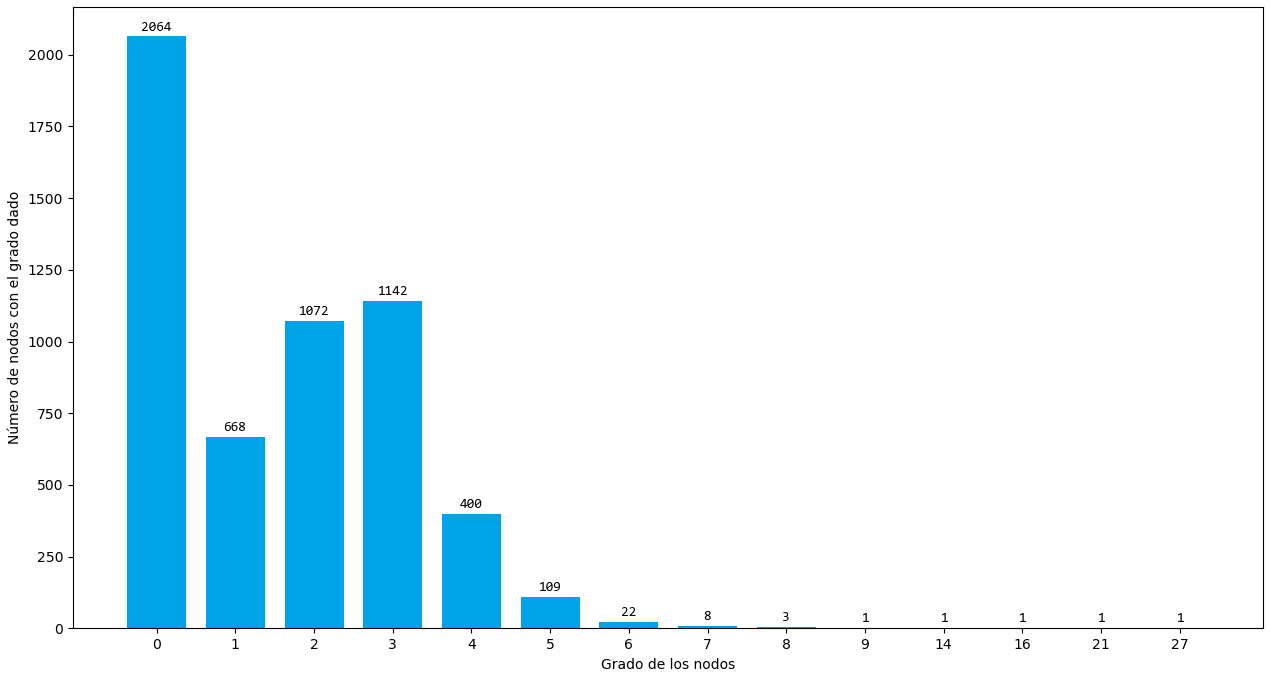
\includegraphics[width=\textwidth]{graphics/degree1.png}
		\caption[Grado de salida de los nodos del grafo]{Grado de salida de los nodos del grafo.}
		\label{fig:out_degree_all_nodes}
	\end{center}
\end{figure}

En la figura \ref{fig:in_degree_all_nodes} se evidencia una relación entre el grado de salida de los nodos y la cantidad de estos que tienen un grado específico. Esto representa la cantidad de relaciones como las explicadas en la sección \ref{section:relation_annotation} en las que el nodo es parte derecha (referenciado a través de \texttt{Arg2}).
\begin{figure}[H]
	\begin{center}
		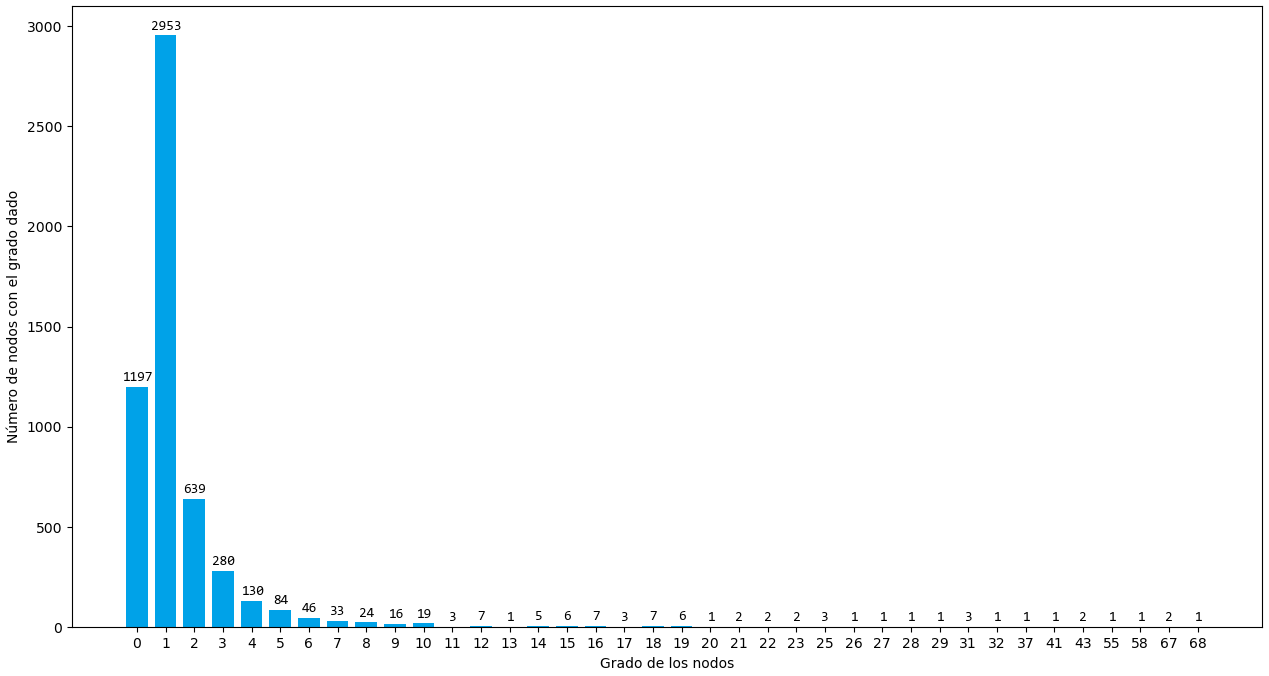
\includegraphics[width=\textwidth]{graphics/degree2.png}
		\caption[Grado de entrada de los nodos del grafo]{Grado de entrada de los nodos del grafo.}
		\label{fig:in_degree_all_nodes}
	\end{center}
\end{figure}

En la figura \ref{fig:out_degree_nodes_by_rol} se evidencia una relación entre el grado de salida de los nodos y la cantidad de estos que tienen un grado específico, pero esta vez agrupados por su rol semántico. Esto representa la cantidad de relaciones como las explicadas en la sección \ref{section:relation_annotation} en las que el nodo es parte izquierda (referenciado a través de \texttt{Arg1}).
\begin{figure}[H]
	\begin{center}
		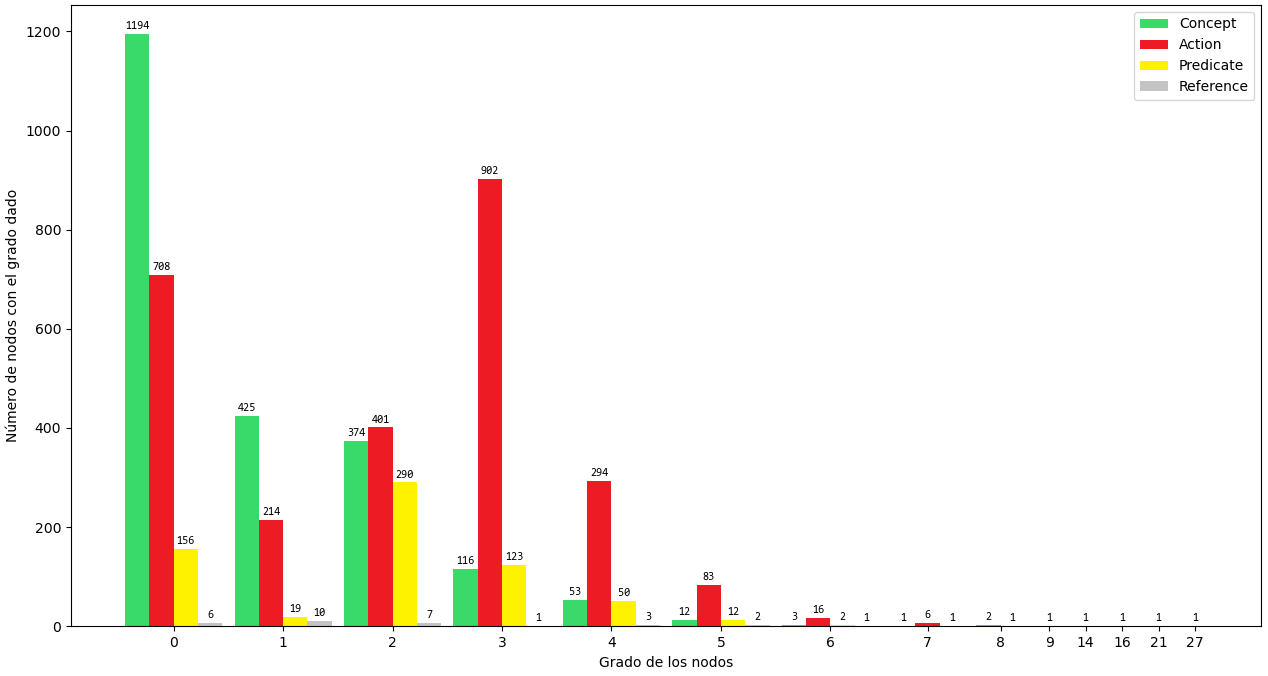
\includegraphics[width=\textwidth]{graphics/degree3.png}
		\caption[Grado de salida de los nodos del grafo por rol]{Grado de salida de los nodos del grafo por rol.}
		\label{fig:out_degree_nodes_by_rol}
	\end{center}
\end{figure}

En la figura \ref{fig:in_degree_nodes_by_rol} se evidencia una relación entre el grado de salida de los nodos y la cantidad de estos que tienen un grado específico, pero esta vez agrupados por su rol semántico. Esto representa la cantidad de relaciones como las explicadas en la sección \ref{section:relation_annotation} en las que el nodo es parte derecha (referenciado a través de \texttt{Arg2}).
\begin{figure}[H]
	\begin{center}
		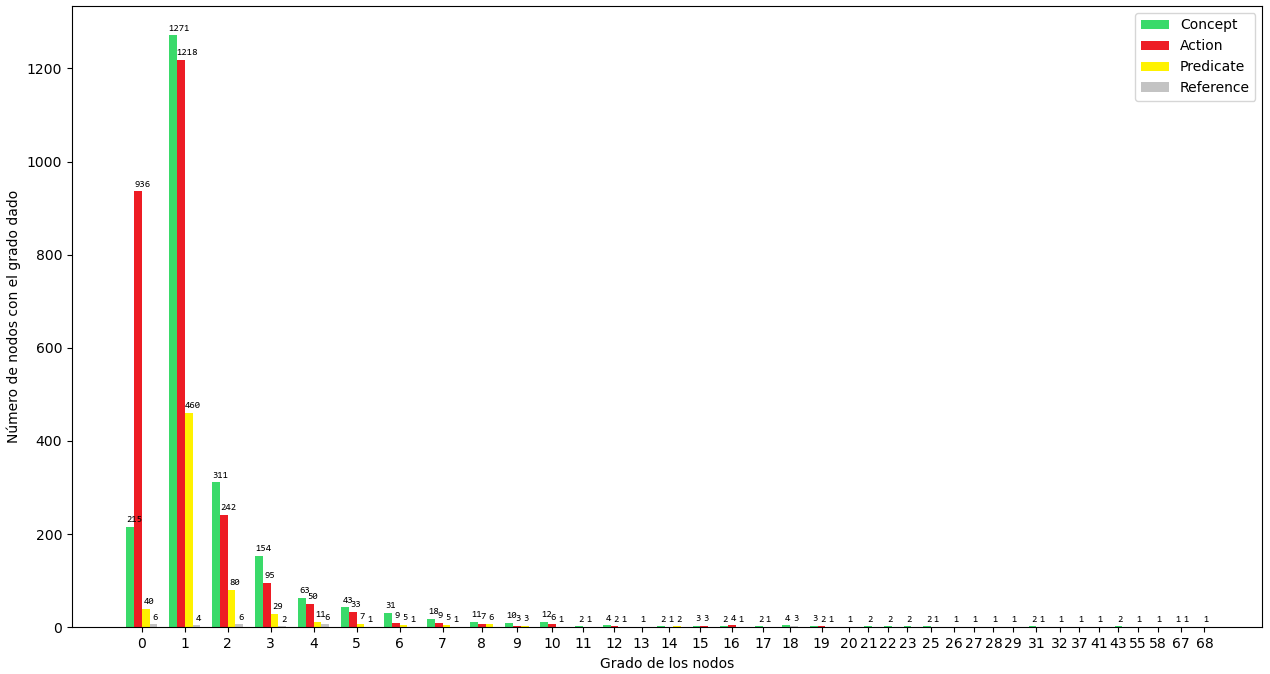
\includegraphics[width=\textwidth]{graphics/degree4.png}
		\caption[Grado de entrada de los nodos del grafo por rol]{Grado de entrada de los nodos del grafo por rol.}
		\label{fig:in_degree_nodes_by_rol}
	\end{center}
\end{figure}

En la tabla \ref{tab:knowledge_graph_stats} se aprecia la cantidad de nodos y aristas según su tipo y a la misma vez se comparan los resultados obtenidos sin normalizar y normalizando las palabras respectivamente. La última columna representa el porcentaje de disminución en cada fila luego de normalizar.
%Esto posibilita una mayor coincidencia de las palabras o frases y por ende, es ideal para una mejor representación y extracción del conocimiento.
\begin{table}[H]
	\begin{center}
		\begin{tabular}{lccc}
			\noalign{\hrule height 1pt}\\
			\vspace{-0.35in}\\
			\textbf{Métrica} & \textbf{Sin normalizar} & \textbf{Normalizando} & \textbf{\% disminuido}\\
			\hline\\
			\vspace{-0.35in}\\
			Conceptos & $5,493$ & $4,935$ & $\approx10.16$\\
			\quad \texttt{Concept} & $2,181$ & $1,969$ & $\approx9.72$\\
			\quad \texttt{Action} & $2,625$ & $2,335$ & $\approx11.05$\\
			\quad \texttt{Reference} & $35$ & $21$ & $40$\\
			\quad \texttt{Predicate} & $652$ & $610$ & $\approx6.44$\\
			\hline\\
			\vspace{-0.35in}\\
			Relaciones & $8,682$ & $8,623$ & $\approx0.68$\\
			\quad \texttt{Concept} & $530$ & $525$ & $\approx0.94$\\
			\quad \texttt{Reference} & $9$ & $9$ & $0$\\
			\quad \texttt{Action} & $1,902$ & $1,875$ & $\approx1.42$\\
			\quad \texttt{Subject} & $923$ & $922$ & $\approx0.11$\\
			\quad \texttt{Target} & $1,572$ & $1,568$ & $\approx0.25$\\
			\quad \texttt{Predicate} & $501$ & $496$ & $\approx1$\\
			\quad \texttt{Domain} & $298$ & $296$ & $\approx0.67$\\
			\quad \texttt{Argument} & $308$ & $307$ & $\approx0.32$\\
			\quad \texttt{Is-a} & $492$ & $481$ & $\approx2.24$\\
			\quad \texttt{Part-of} & $89$ & $89$ & $0$\\
			\quad \texttt{Same-as} & $231$ & $231$ & $0$\\
			\quad \texttt{Has-property} & $143$ & $143$ & $0$\\
			\quad \texttt{Causes} & $360$ & $360$ & $0$\\
			\quad \texttt{Entails} & $200$ & $199$ & $0.5$\\
			\quad \texttt{In-time} & $154$ & $154$ & $0$\\
			\quad \texttt{In-place} & $361$ & $360$ & $\approx0.28$\\
			\quad \texttt{In-context} & $609$ & $608$ & $\approx0.16$\\
			\hline\\
			\vspace{-0.35in}\\
			Atributos & $359$ & $329$ & $\approx8.36$\\
			\quad \texttt{Negated} & $111$ & $94$ & $\approx15.32$\\
			\quad \texttt{Uncertain} & $150$ & $141$ & $6$\\
			\quad \texttt{Diminished} & $83$ & $80$ & $\approx3.61$\\
			\quad \texttt{Emphasized} & $15$ & $14$ & $\approx6.67$\\
			\noalign{\hrule height 1pt}
		\end{tabular}
		\caption[Estadísticas del grafo de conocimiento]{Estadísticas del grafo de conocimiento.}
		\label{tab:knowledge_graph_stats}
	\end{center}
\end{table}

Como se ha podido observar anteriormente, una de las principales funciones de las ontologías y los grafos de conocimiento es la extracción de conocimiento que no está representado explícitamente en el corpus. Un ejemplo de ello es:

\begin{table}[H]
	\begin{center}
		\begin{tabular}{cc}
			\noalign{\hrule height 1pt}\\
			\vspace{-0.35in}\\
			\textbf{Documento} & \textbf{Relación explícita}\\
			\hline\\
			\vspace{-0.35in}\\
			\texttt{cirugía.ann} & \guillemot{\texttt{cirugía de corazón} \textit{is-a} \texttt{operación}}\\
			\texttt{hígado graso.ann} & \guillemot{\texttt{operación} \textit{is-a} \texttt{procedimiento médico}}\\
			\noalign{\hrule height 1pt}\\
			\vspace{-0.35in}\\
			& \textbf{Relación implícita}\\
			& \guillemot{\texttt{cirugía de corazón} \textit{is-a} \texttt{procedimiento médico}}\\
			\noalign{\hrule height 1pt}
		\end{tabular}
		\caption[Ejemplo de extracción de conocimiento implícito]{Ejemplo de extracción de conocimiento implícito.}
		\label{tab:implicit_knowledge_extraction}
	\end{center}
\end{table}

\section{Discusión}
Todos los nodos del grafo de conocimiento participan en al menos una relación, pero como se aprecia en las figuras \ref{fig:out_degree_all_nodes}, \ref{fig:in_degree_all_nodes}, \ref{fig:out_degree_nodes_by_rol} y \ref{fig:in_degree_nodes_by_rol}, hay muchos nodos que tiene un grado bajo. En el caso en que la gráfica muestra la cantidad de nodos con grado cero, esto viene dado o bien porque ese nodo no tiene relaciones de salida y en este caso tendría grado de salida cero o bien no tiene relaciones de entrada y por tanto grado de entrada cero. El hecho de que pocos nodos tengan un alto grado viene dado porque usualmente los nodos más grandes y con más palabras, al ser conocimiento más específico participan en un menor número de relaciones.

Los roles semánticos \textit{Concept} y \textit{Action} que participan en una mayor cantidad de relaciones en este grafo de conocimiento son \guillemot{\texttt{persona}} y \guillemot{\texttt{tratamiento}} respectivamente. Dado que se trabajó con un corpus de documentos médicos, este resultado cobra sentido pues esas palabras son ampliamente empleadas en este medio.

En la tabla \ref{tab:knowledge_graph_stats} se muestra el resultado de un grafo de conocimiento utilizando palabras o frases sin normalizar y normalizadas. Normalizar las palabras no solo reduce la cantidad de nodos y aristas en el grafo sino que también potencialmente aumenta la cantidad de conocimiento implícito que se puede extraer. Esto sucede debido a que en el grafo, todas las relaciones explícitamente escritas en el corpus representan dos nodos y una arista entre estos. Por tanto, si dos nodos no tienen aristas entre ellos, pero existe un camino que los conecta, esto es conocimiento implícito descubierto a través del grafo.

El hecho de normalizar implica, por ejemplo, que todas las conjugaciones de un mismo verbo deben resultar en el verbo sin conjugar. Esto trae consigo muchas ventajas, puesto que todas las relaciones de entrada y salida de ese grupo de palabras quedan contenidas en una única palabra y por ende, puede ampliar potencialmente la cantidad de caminos en el grafo y con ello, la cantidad de conocimiento ímplicito extraído.

Una deficiencia clara sucedió a la hora de hallar los resultados de la tabla \ref{}. Para este tipo de evaluación, lo ideal es tener un grafo de conocimiento formado a partir de una ontología y de un corpus preferentemente grande. A su vez, el grafo debe ser revisado con otro corpus perteneciente al mismo tema y de mediano o gran tamaño. Muchas veces esto es difícil de lograr, y en efecto, es lo que sucedió. Para llevar a cabo esta tarea, se dividieron las oraciones anotadas en dos grupos, un grupo de \textit{training} (\textit{entrenamiento} en español) con el cual se realizará el grafo de conocimiento y un grupo de \textit{testing} (\textit{prueba} en español), con el que se revisará la existencia de las anotaciones de texto y las relaciones respecto a las que ya están construidas en el grafo.